\section{Framework Concept}

\subsection{Introduction}

The Golem System is a framework for trading computing power in the Peer2Peer (P2P) model.
Settlement of computing power usage takes place in the Etherium network and its derivatives.

The framework consists of a set of basic components and dependencies between them, 
as well as programming elements that allow for the creation of decentralized and distributed
applications and services using the Golem trading model.

These are:

\begin{itemize}

\item protocols
\item libraries
\item API
\item implementation of sample components

\end{itemize}

The goal of the Golem System is to provide

\begin{itemize}

\item portability
\item ease of installation
\item flexibility

\end{itemize}

In this chapter, the general concept of the Golem network architecture will be presented. 
Both the assumptions and elements of the network, applications, services, protocols will be 
described in the most abstract way possible, so as not to lose the idea of ​​solving the system 
due to the complexity of the processes taking place in it.

A detailed description of the components will be described later in the document.

%\subsection{Definitions}
%\begin{description}
%\item[Plane] This is a set of elements (physical, virtual or their abstractions),
%applications, services, protocols, functions that allow for internal
%and external communication, their configuration and monitoring at all layers.
%\end{description}

\newpage

\subsection{Abstract Architecture}

The architecture of the Golem System will be presented on three planes 
(Please see Figure ~\ref{fig:Plane} on page ~\pageref{fig:Plane}):

\begin{enumerate}
	\item Golem Plane (GP)
	\item User Plane (UP)
	\item External Provider Plane (EPP)
\end{enumerate}

\begin{figure}[htbp]
    \centering
    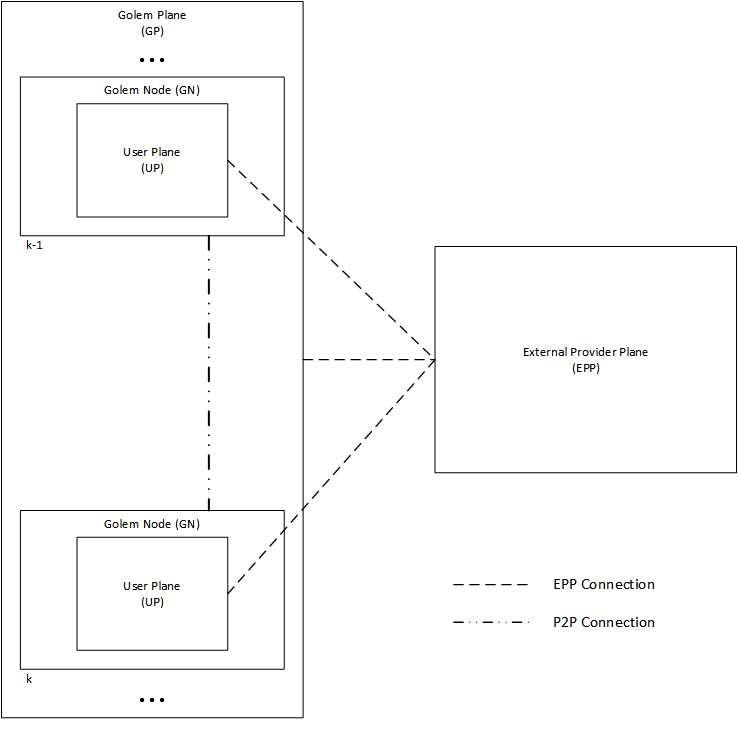
\includegraphics[width=8cm,height=8cm,angle=0]{./diag/Abstract/GolemSystemPlane-Abstract.png}
    \caption{Abstraction Plane Concept}
	\label{fig:Plane}
\end{figure}

The Golem Plane is the basis on which nodes called Golem Nodes are defined, which build the Golem Network 
(Please see Figure ~\ref{fig:Ntw} on page ~\pageref{fig:Ntw}).

\begin{figure}[htbp]
    \centering
    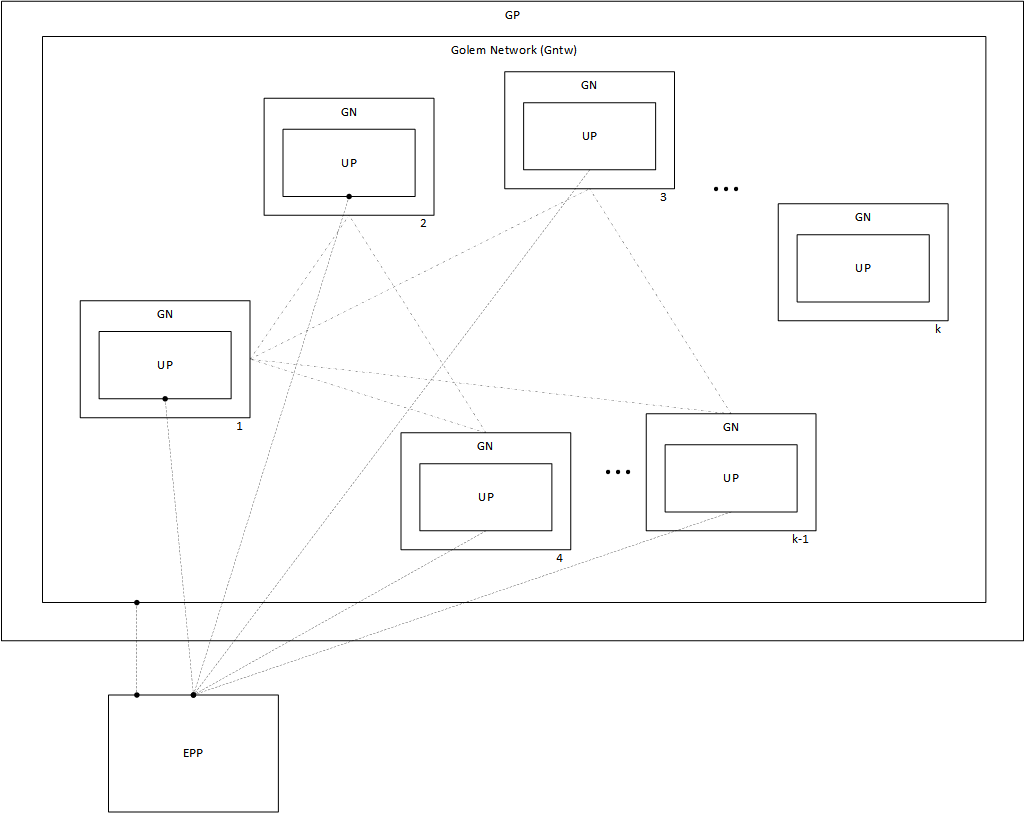
\includegraphics[width=8cm,height=8cm,angle=0]{./diag/Abstract/GolemSystemNetwork-Abstract.png}
	\caption{Abstraction Network Concept}
    \label{fig:Ntw}
\end{figure}

Each node consists of a set of core applications, core services
and core protocols enabling communication, configuration and monitoring 
on all layers of decentralized and distributed business processes.
Business processes are implemented on the User Plane using functions of 
core components of applications, services and protocols through their API.
The External Operator Plane is used for specific functions implemented
outside the Golem Network but used by this network. An example is the availability of
payments in cryptocurrencies.

The above Planes with their component elements distributed over three main layers 
are shown in the figure (Please see Figure ~\ref{fig:Arch} on page ~\pageref{fig:Arch}):

\begin{enumerate}
	\item Platform Layer (PL)
	\item Integration Layer (IL)
	\item Buisness Layer (BL)
\end{enumerate}

In the Platform Layer (PL) there is the Golem Agent (GA) element,
which allows you to create a Golem Node (GN) from a computer unit.
Golem Node is a member of the Golem Network (Gntw).

In the Integration Layer (IL) there is the Golem Agent console (GAC) and Golem Toolkit (GTK).
The Golem Agent console consists of tools for configuring and monitoring the created applications and services
and managing the Golem Agent element, which is a daemon of the created node (GN).
The Golem Toolkit is a set of tools, APIs that allow you to create decentralized and distributed applications and services
on the Golem network infrastructure and using the Golem commercial model.

In the Business Layer (BL) there is the user plane (UP) and the external provider plane (EPP).

In the user plane (UP), decentralized applications and services of the Golem network are implemented.
Users can use service and application templates created in the form of the "standards - change the name" framework specification.

This layer defines user roles that can be assigned to Golem nodes depending on the aspect of the node's computational resources and/or the service it provides.

The external provider layer (EPP) is used to handle payments that take place on the Etherium network and its derivatives.
This layer can be used to define and implement connections to other application and service networks.

\afterpage{
\begin{landscape}
	\begin{figure}[htbp]
		\centering
		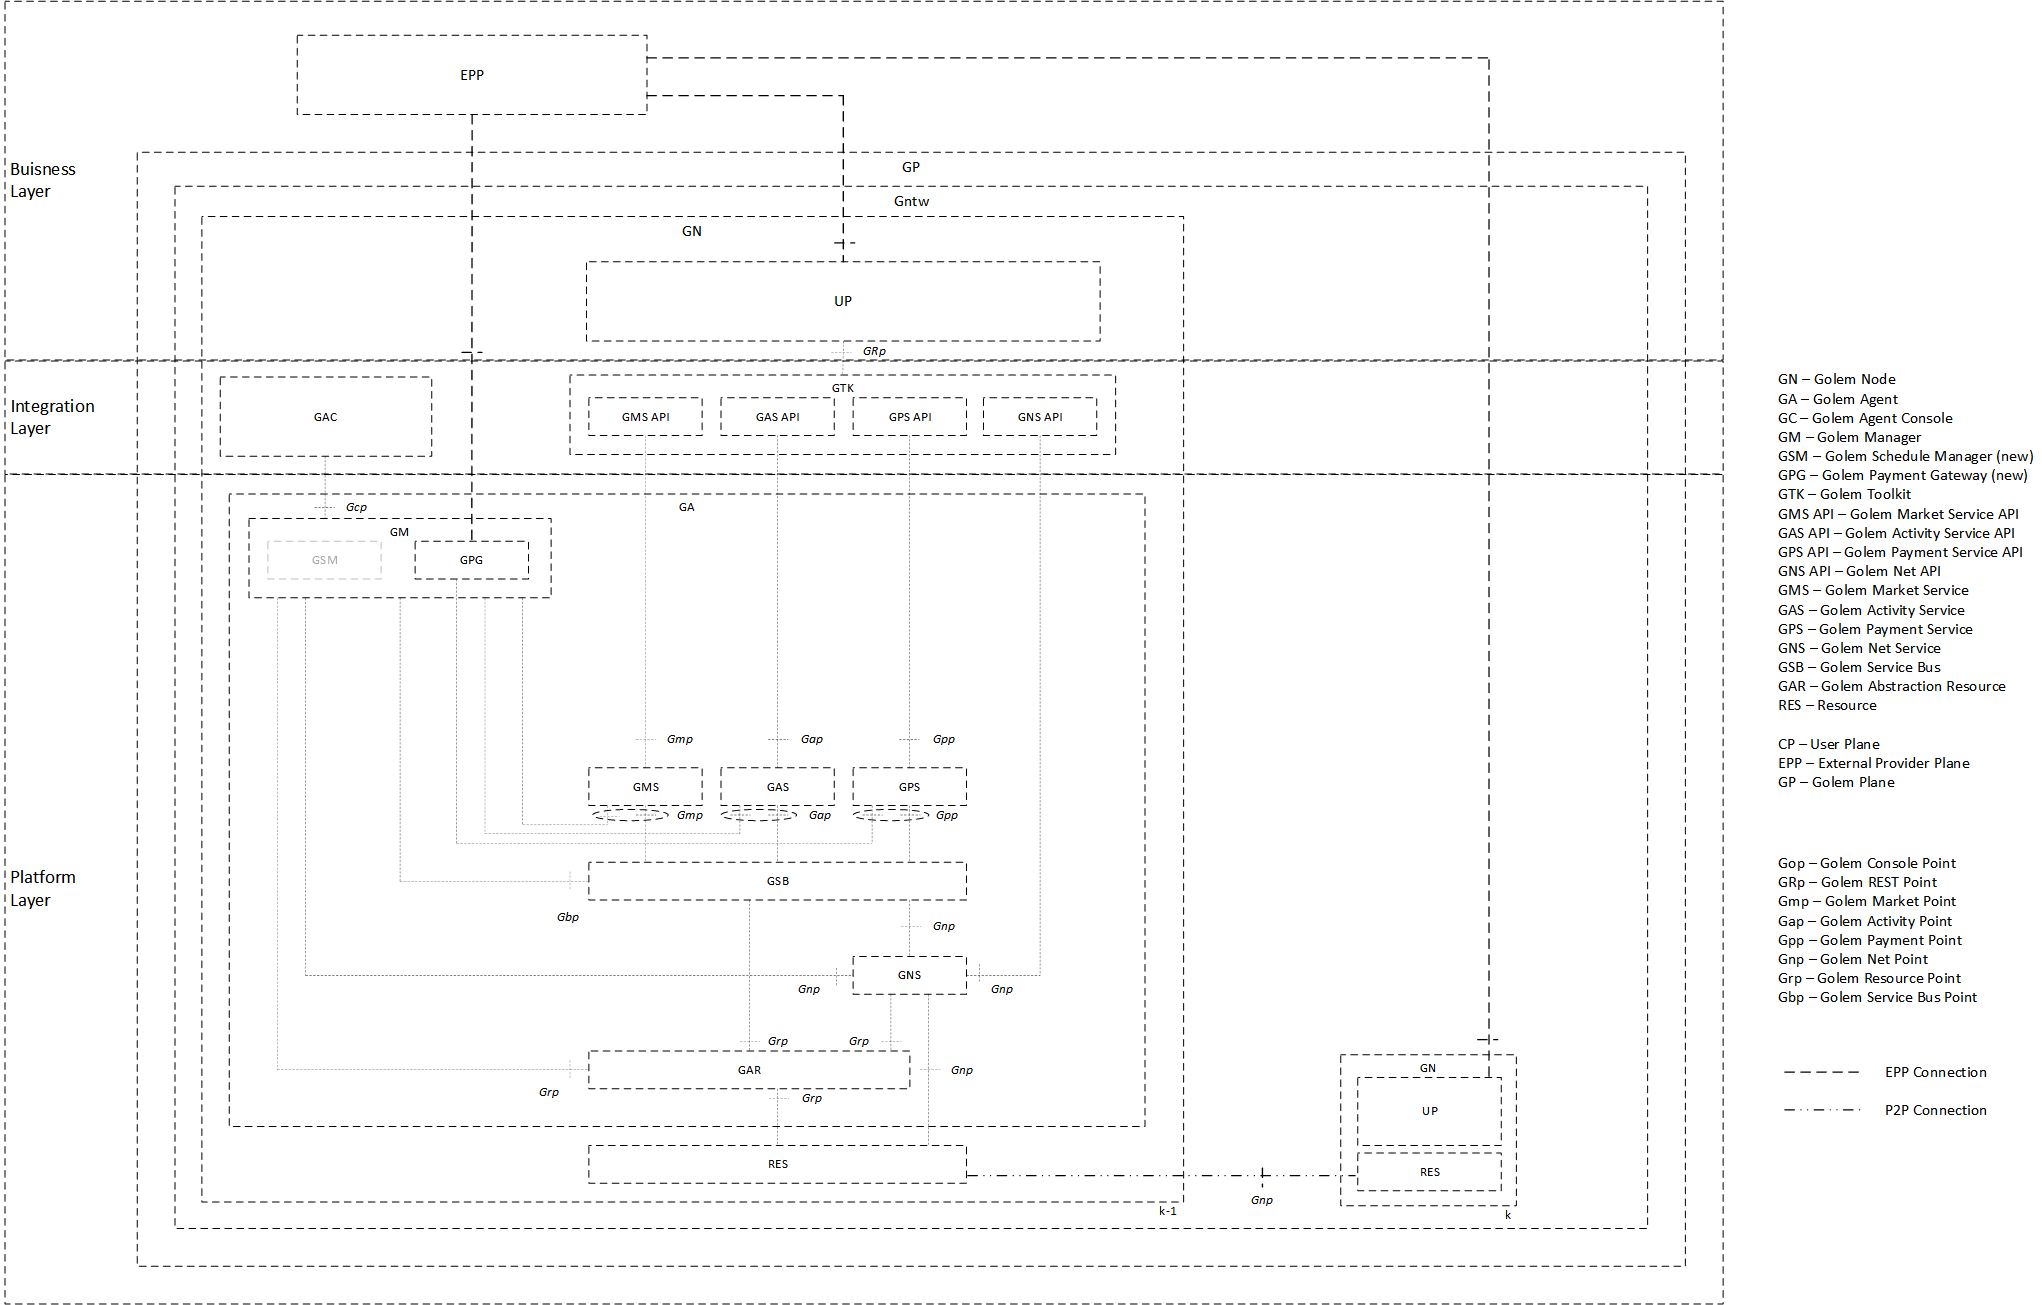
\includegraphics[width=\hsize]{./diag/Abstract/GolemSystemLayers-Abstract.png}
		\caption{Abstraction Architecture Diagram}
		\label{fig:Arch}
	\end{figure}
\end{landscape}
}

\newpage

The subject of the trade (purchase-sale of the service of using computing resources)
is described using the service model description language (Golem SMDL).
This language is based on a simple definition of resource parameters (the list is available) and their constraints, which are expressed using filters.
The filter syntax is based on the LDAP filter syntax.

The general description of the service should include:

\begin{itemize}
\item {\bf Resource vector R} describes the infrastructure environment using qualitative and quantitative parameters as a service being traded
\item {\bf Usage vector B} defines the factors influencing the measurement of the consumption of the service of using computing resources. These factors are expressed in arbitrary counters
\item {\bf Context vector C} includes important factors that affect the price
\item {\bf Pricing function} indicates the service parameters and cumulative usage counters that affect the cost of the service
\end{itemize}

The following parties participate in the trading process

\begin{itemize}
\item {\bf requestor :} a role of a P2P network node that wants to use the computing resources of other nodes.
\item {\bf provider :} a role of a P2P network node that wants to sell its resources to other nodes
\item {\bf user :} an end user who represents the requestor node and/or the provider
\item {\bf developer :} an application developer
\end{itemize}

A user as a provider prepares an offer in the form of an Offer object using the service model description language.
A user as a requestor prepares a demand in the form of a Demand object using the service model description language.
Both the Offer and Demand objects consist of two elements:

\begin{itemize}
\item properties
\item constraints
\end{itemize}

The formal language of resource description and settlement conditions is intended to automatically or semi-automatically associate demands with offers.
The specification of the service model description language is presented later in the document.

\newpage

%A single aspect of a resource and/or service defines a dimension of the namespace.
% Thus, a set of dimensions creates a multidimensional structure of the namespace.
%Golem Agent contains basic tools for creating a decentralized market of distributed applications and services. These are:
%\begin{enumerate}
%\item {\bf Golem Market Service (GMS)}
%\item {\bf Golem Activity Service (GAS)}
%\item {\bf Golem Payment Service (GPS)}
%\item {\bf Golem Net Service (GNS)
%\item {\bf Golem Services API}
%The following APIs are available:
%\begin{itemize}
%\item Golem Market Service API (GMS API)
%\item Golem Activity Service API (GAS API)
%\item Golem Payment Service API (GPS API)
%\item Golem Net Service API (GNS API)
%\item Golem Service Bus API (GSB API)
%\end{itemize}
%All of the above services have APIs that allow you to create new decentralized and distributed applications and services,
%which use the created Golem network infrastructure (Gntw) and the genericity properties of the underlying services.
%The APIs of individual services also allow you to create interaction automation, e.g. settlements, 
%and offer optimization and orders, and many other tools.
%\end{enumerate}

%\break

%\subsection{Reference Architecture}